\usetikzlibrary{arrows.meta}
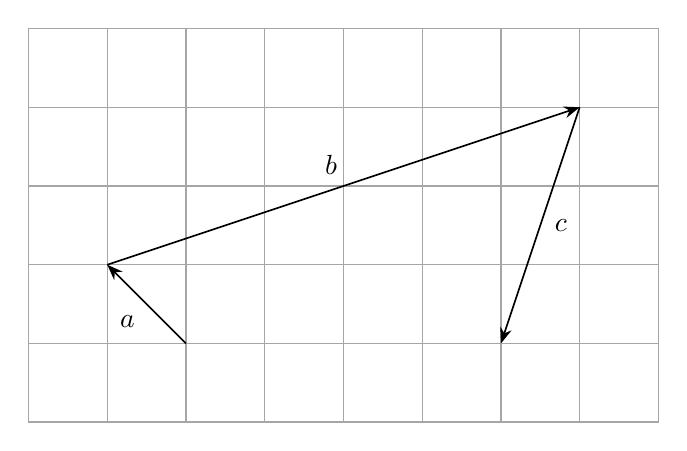
\begin{tikzpicture}[x=10mm,y=10mm,line width=.6pt,font=\normalsize,>=Stealth]
\tikzset{vec/.style={draw=black,line width=.6pt,->,>=Stealth}}
\draw[draw=gray!70,line width=.45pt] (0,0) grid[xstep=1,ystep=1] (8,5);
\draw[draw=gray!70,line width=.6pt] (0,0) rectangle (8,5);
\draw[vec] (2,1) -- (1,2);
\draw[vec] (1,2) -- (7,4);
\draw[vec] (7,4) -- (6,1);
\node[inner sep=0pt,anchor=north east,xshift=-4pt,yshift=-4pt] at (1.5,1.5) {$\symbfit{a}$};
\node[inner sep=0pt,anchor=south east,xshift=-2pt,yshift=4pt] at (4,3) {$\symbfit{b}$};
\node[inner sep=0pt,anchor=west,xshift=5pt] at (6.5,2.5) {$\symbfit{c}$};
\end{tikzpicture}
